\documentclass{article}
\usepackage[a4paper, total={6in, 8in}, margin=0.8in]{geometry}
\usepackage{textcomp}
\usepackage{gensymb}
\usepackage{amsfonts}
\usepackage{amsmath}
\usepackage{graphicx}
\graphicspath{ {.} }

\begin{document}

\begin{titlepage}
    \vspace*{\fill}
    \begin{center}
        {\Huge\bfseries Projeto BD - Parte 1\\}
        \vspace{1cm}
        {\Large\bfseries Francisco Fonseca -- 102492}\\[5pt]
        $33.(3)\%$ (3 horas)\\[14pt]
        {\Large\bfseries Gonçalo Rua -- 102604}\\[5pt]
        $33.(3)\%$ (3 horas)\\[14pt]
        {\Large\bfseries João Gouveia -- 102611}\\[5pt]
        $33.(3)\%$ (3 horas)\\[14pt]
    \end{center}
    \vspace*{\fill}

    \vspace{0.5cm}

    \begin{itemize}
        \item[] \Large\bfseries Grupo: 10
        \item[] \Large\bfseries Turno: BD2L12
        \item[] \Large\bfseries Professor: Flávio Martins
    \end{itemize}

\end{titlepage}

\section{Diagrama de modelo de Entidade-Associação}

\vspace{0.5cm}
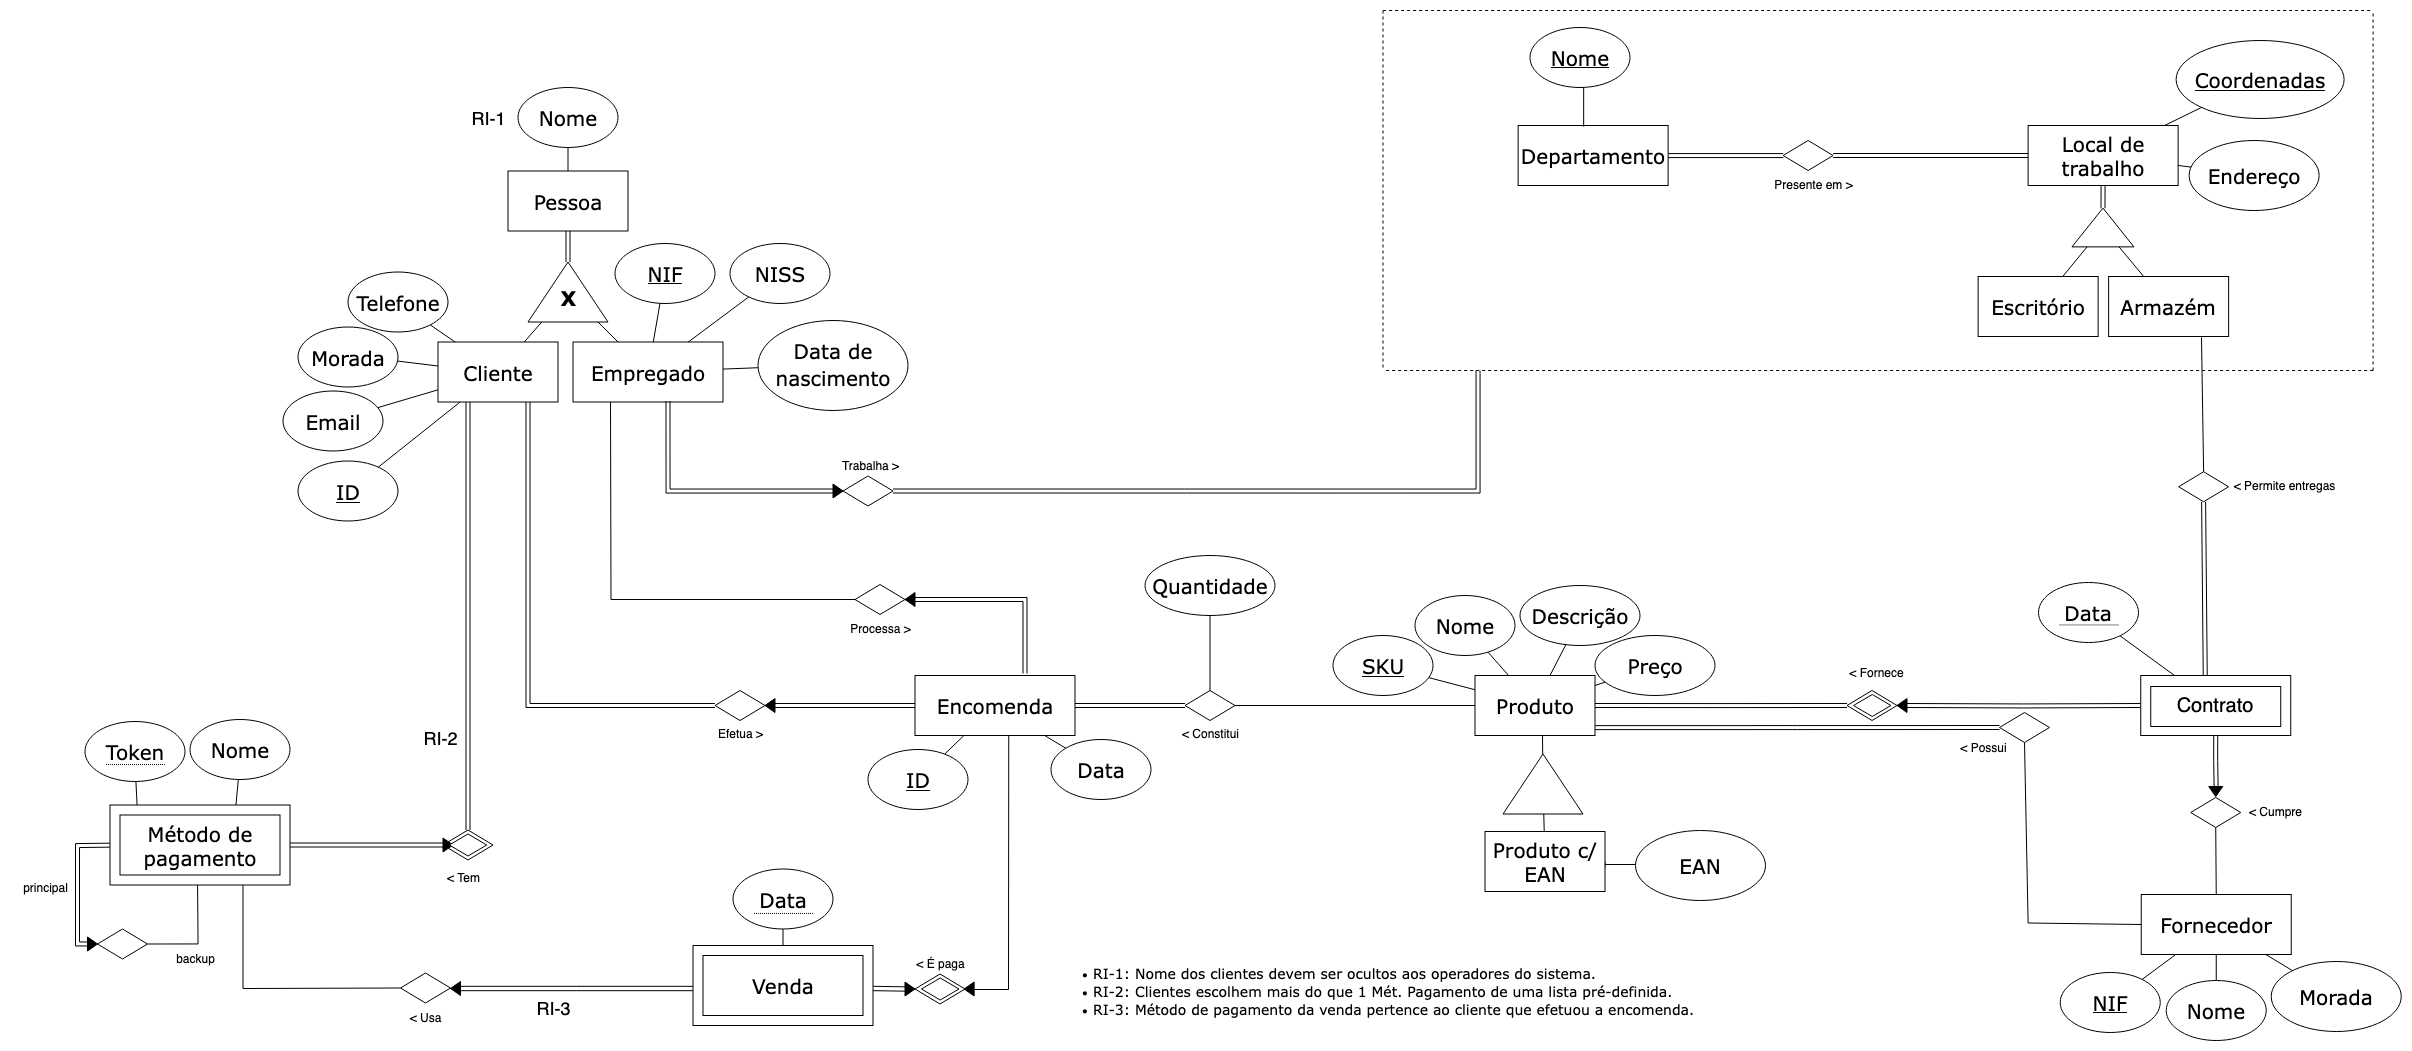
\includegraphics[scale=0.2]{diagrama.png}
\vspace{0.5cm}

\section{Restrições de integridade}

\begin{itemize}
    \item RI-1: Nome dos clientes devem ser ocultos aos operadores do sistema.
    \item RI-2: Clientes escolhem mais do que 1 Mét. Pagamento de uma lista pré-definida.
    \item RI-3: Método de pagamento da venda pertence ao cliente que efetuou a encomenda.
\end{itemize}

\end{document}